\subsection{Vorbereitungen 13.07.2011}
Da ich am Abend eingeladen war,  bei einer Elektroinstallation zu helfen, ergriff ich gleich die Chance und holte den Bus, um am Freitag pünktlich an das Geburtstags-Essen zu kommen.

\subsection{Freitag 15.07.2011}
Eigentlich wollte im den Nachmittag frei nehmen, um zu packen und den Bus zu beladen.
Jedoch waren da noch zwei Testflüge im Weg und so wurde es nach 17 Uhr bis ich die Flugzeugwerke in Stans verlassen konnte.
Gerade so schaffte ich es zum Nachtessen in der Seerose.
Nach einem feinen Nachtessen musste also noch unser ganzer Karsumpel eingepackt werden.
Die spontan eintretende Müdigkeit machte das unterfangen nicht gerade leichter und auch der Wetterbericht verhiess nichts Gutes für die kommenden
Tage.
Diese Vorhersage bedeutete, dass eher noch mehr Material den Weg in den Bus finden musste.

\subsection{Samstag 16.07.2011}
\begin{wrapfigure}{R}{0.45\textwidth} 
  \begin{centering}
    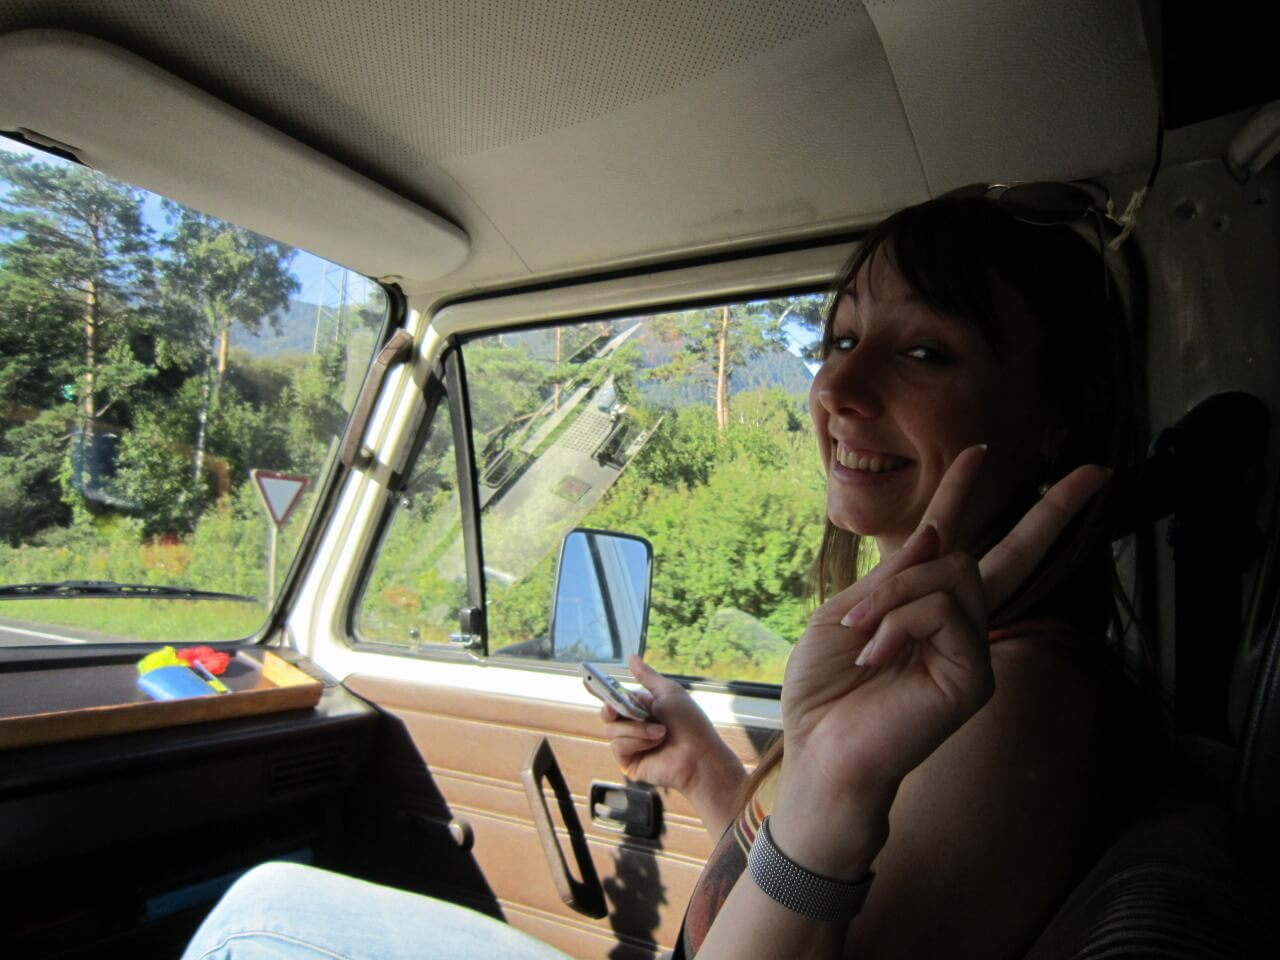
\includegraphics[width=0.4\textwidth, height=5cm, keepaspectratio]{../Bilder/Locarno/3.jpg}
    \caption{Ab in den Süden}
  \end{centering}
\end{wrapfigure} 

Nach einer viel zu kurzen Nacht hiess es um kurz nach 5 Uhr ab auf die Füsse.
Mir fiel es nicht gerade schwer aufzustehen, da mein Magen das klare Kommando zum entleeren seiner selbst gegeben hat.
Ich bekam die volle Wucht des gefürchteten Nachbrandes nach dem Genuss von scharfem Essen zu spüren.
Nach kurzer Zeit war es relativ ruhig im Bus und alle Beifahrer schlummerten und träumten von Sonne, Strand und Jack Johnson.
Kaum auf die Westumfahrung aufgefahren, machte uns eine grosse Tafel darauf aufmerksam,
unsere geplante Route durch den Gotthard zu verlassen und dem San Bernadino einen Besuch abzustatten.
Nach kurzer Recherche konnte uns das Argument von fast zwei Stunden Wartezeit überzeugen und so ging es Richtung Chur dem San Bernadino entgegen.
Der obligate Halt im Heidiland verbrachten wir mit Diskussionen über die WC- Bons und natürlich kam gerade vor uns ein Car mit einer ganzen Ladung Blumenkohl an, welche erbarmungslos alle verfügbaren Kassen verstopften.
Während der weiteren Fahrt gen
Süden verpasste Chantal so ziemlich alle schönen Sujet beim Studium der Bedienungsanleitung ihrer neuen Kamera.
Die Ersatzbank war eh schon länger am dösen und nickte im Takt der Fahrbahnunebenheiten.
Im gelobten Tessin angekommen, forderte uns das Navi mit einer Strasse von 1.5 Fahrbahnbreiten heraus.
Schon bald kamen wir dann auf dem Camping Delta an.
Die zuerst unfreundliche Dame am Schalter bestand darauf, dass ich ihr persönlich meinen Ausweis unter ihre Nase halte.
Als Michel und ich vor ihrem Häuschen auftauchten, verbesserte sich ihre Laune schlagartig.
Der Platz war schnell gefunden und unsere zwei Untermieter machten sich sofort daran ihr neues Zuhause aufzustellen.
Kaum stand das mobile Heim war auch schon der Teufel los und es regnete wie es nur im Tessin seichen kann.
Glücklicherweise besserte sich das Wetter wieder und der kleinen Ausfahrt ins Maggia Tal stand nichts mehr im Weg.
Je weiter wir dem Tal folgten, desto schlechter wurde das Wetter.
So fanden wir uns bald
darauf wieder auf dem Weg zurück nach Locarno Richtung besseres Wetter.
Ein lauschiges Plätzchen an der Maggia war auch schnell gefunden.
Michel und ich unternahmen eine ausgedehnte Erkundungstour und hüpften gazellenartig geschickt von Stein zu Stein um dem kalten Wasser zu entkommen.
Dank eines netten Nachbarn entstand ein Gruppenfoto.
Es wird gemunkelt, dass gewisse Personen nach diesem Foto ihren Psychologen aufsuchen müssen um die schrecklichen Bilder aus ihrem Kopf zu verbannen.
Der nette Fotograf parkte sein nur durch feine, hautenge Badehosen bedecktes Gehänge kniend auf einem Stein vor uns, um einen sicheren \glqq Stand\grqq{} für die Kameraauslösung zu haben.
Die nachfolgende Shoppingtour im Coop gehört in das Kapitel: Geh nie mit Hunger einkaufen.
Der Besuch des angrenzenden Bistros konnte man getrost auf die selbe Ebene wie ein Besuch des Bahnhof Buvette am Samstag Morgen stellen.
Lauter merkwürdige Gestalten mit teils argen modischen Missgeschicken bevölkerten diesen Ort.
Zurück auf dem Campingplatz steigerten wir uns nach einer kurzen Verschnaufpause während dem Apéro in einen wahren Speedmington Rausch.
Da die Flasche Prossecco durchaus Anklang bei der weiblichen Begleitung fand, stieg auch der Lärmpegel und schon bald war dir Umgebung Menschenleer.
Nach einem längeren Ballwechsel war es an der Zeit sich im See abzukühlen.
Hart wie Männer sind, konnten uns auch die vorbeitreibenden Eisberge nicht erschrecken und wir tauchten genüsslich im Lago.
Fabienne krönte das Nachtessen mit ihrer persönlichen Interpretation einer Rahmsauce.
Das Bier verschwand schneller als es aus der Kühlbox getragen werde konnte und so begruben wir schon bald die Idee noch nach Locarno zu \glqq wandern\grqq{}.
Das Bett war zu diesem Zeitpunkt eine viel zu gute Alternative.

\begin{figure}[H]
   \centering
      %\sDas Keyboard 4 Professional	ubfloat[CAPTION]{BILDERCODE}\qquad
   \subfloat{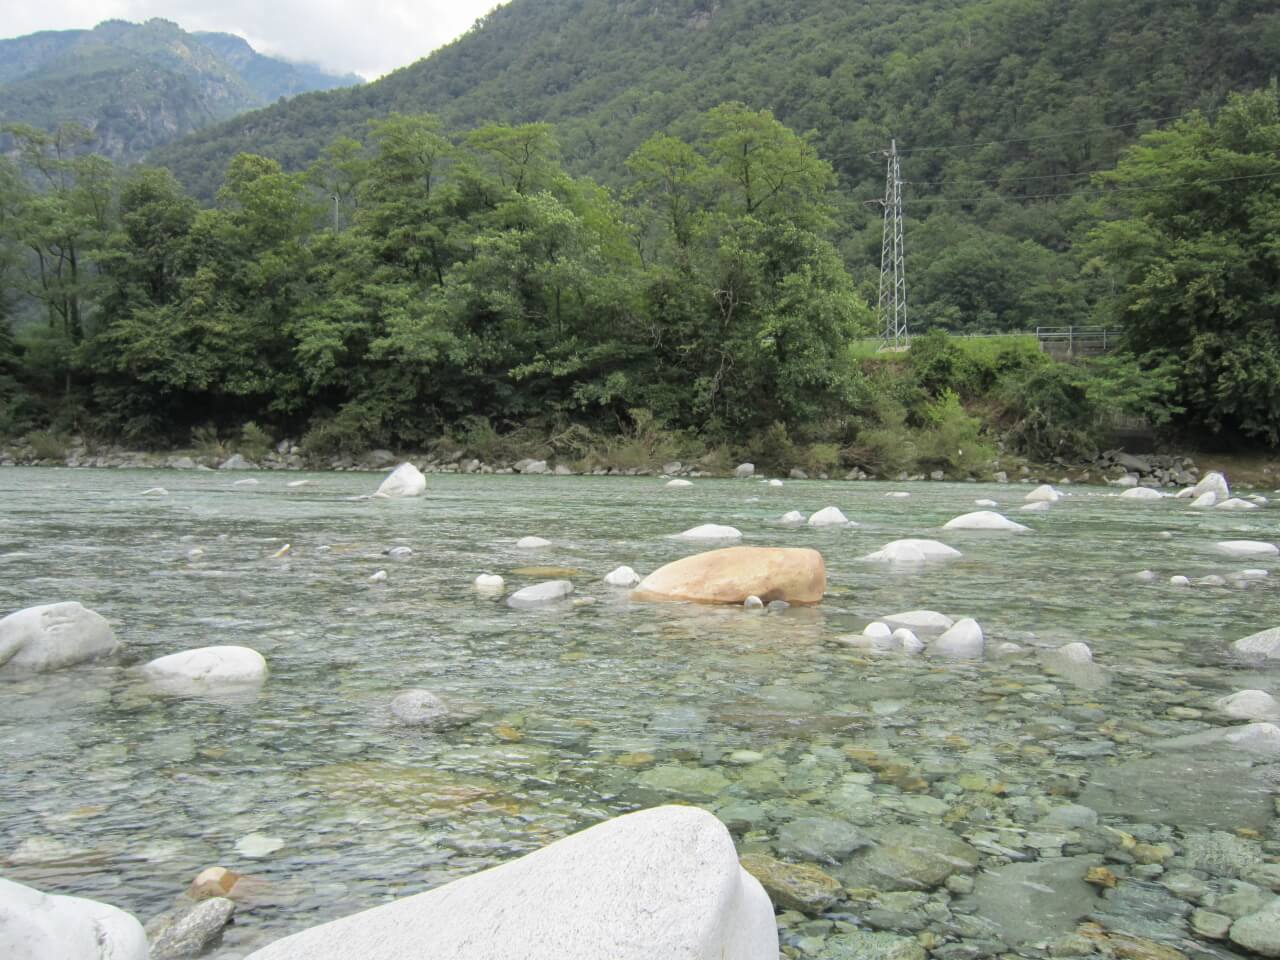
\includegraphics [width=0.3\textwidth]{../Bilder/Locarno/9.jpg}}\quad
   \subfloat{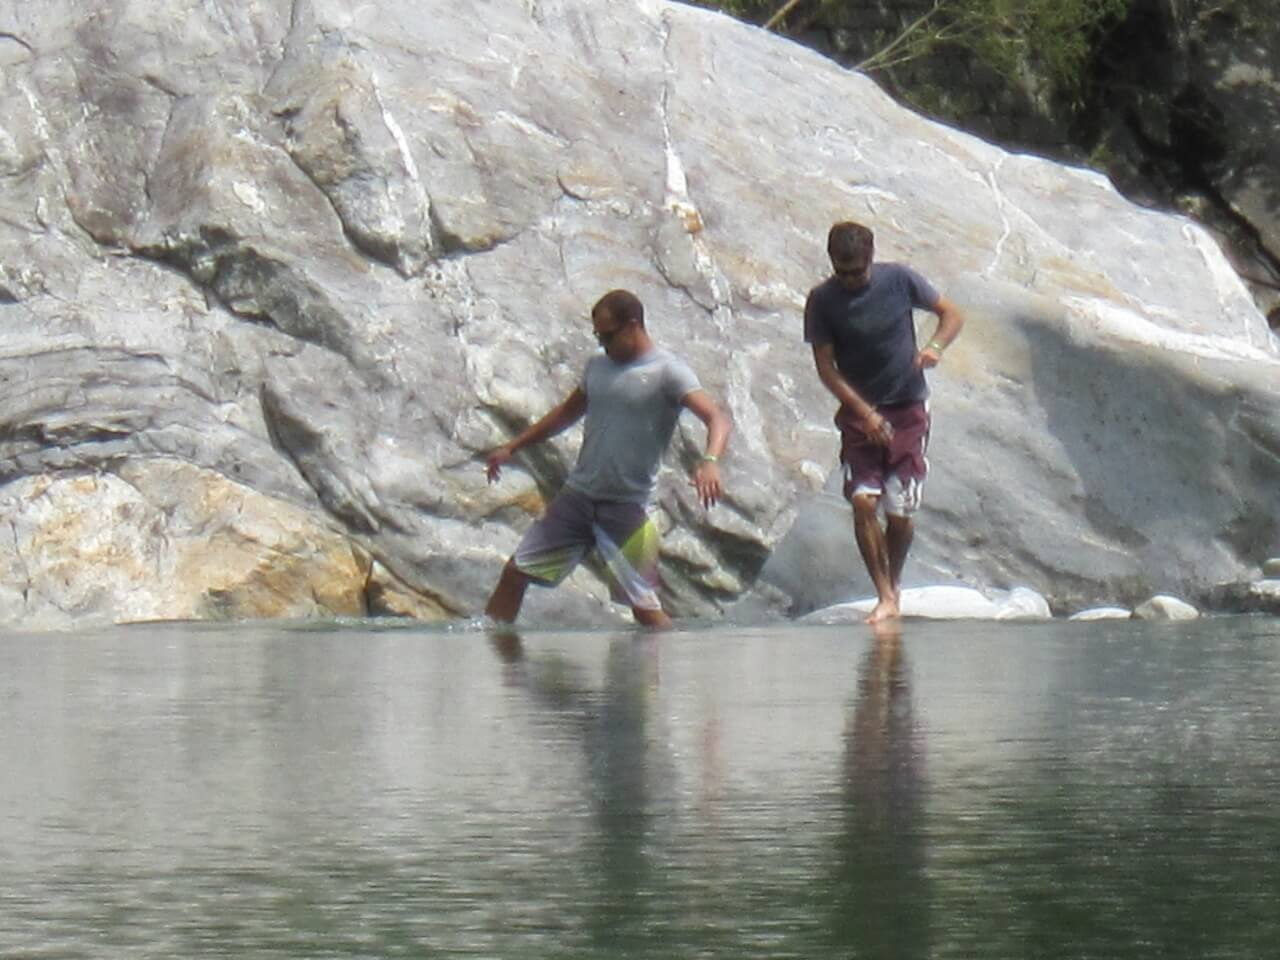
\includegraphics [width=0.3\textwidth]{../Bilder/Locarno/11.jpg}}\quad
   \subfloat{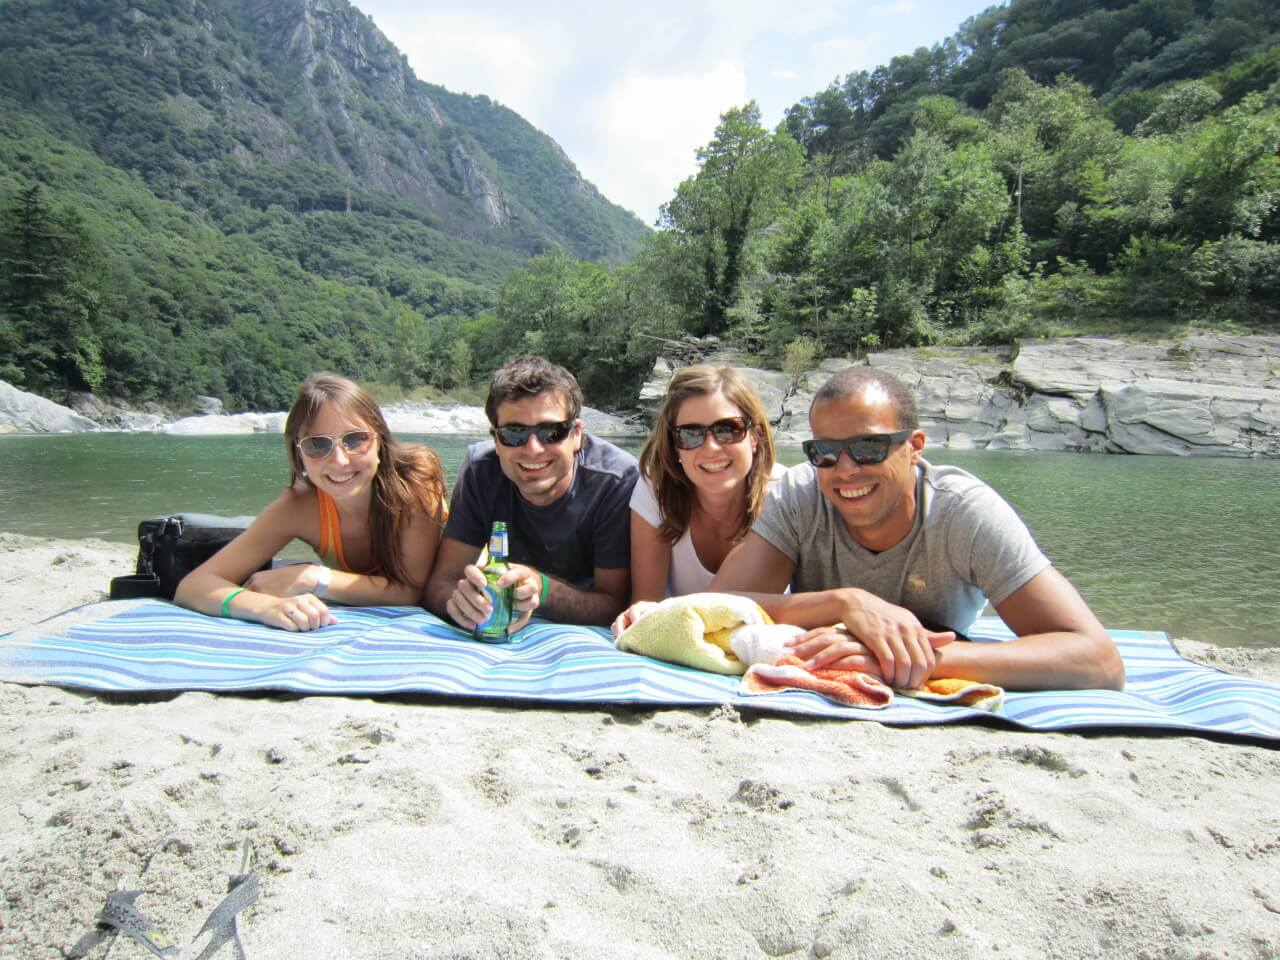
\includegraphics [width=0.3\textwidth]{../Bilder/Locarno/15.jpg}}\quad
   \caption[Action an der Maggia]{Action an der Maggia}
\end{figure}

\subsection{Sonntag 17.07.2011}
Das einheitliche Grau vor dem Fenster liess nichts Gutes erahnen.
Schon während der Nacht wurde alles mit reichlich Wasser begossen.
Irgendwie gelang es uns trotz allem das Frühstück im freien während einer Regenpause zu uns zu nehmen.
Natürlich wuchs der Wunsch nach Cannobio an den berühmt berüchtigten Markt zu gehen.
Die Variante mit dem Schiff in das angrenzende Ausland zu fahren wurde nicht gerade positiv aufgenommen.
Während der kurzen Fahrt öffnete der Himmel alle Schleusen und die Fahrt glich eher einer Bootsfahrt, welche ja kurz vorher noch eher negativ bewertet wurde.
Die Kolonne welche uns Eingangs Cannobio erwartete verhiess nicht Gutes.
Der lokale Sportplatz wird am Sonntag regelmässig zum Parkplatz umgebaut und auch wir stellten den Bus in Mitten von anderen Schweizer Schnäppchenjäger ab.
Zuerst mussten Moneten organisiert werden.
Die Situation ähnelte sehr stark dem Parkplatzproblem.
Die Nachfrage übertraf das Angebot.
Während dem Anstehen bekamen wir aus dem fernen Aargau den Hinweis, dass der Markt nur bis um 13:00 Uhr geöffnet hat.
Es war jedoch schon nach 12:00 Uhr und diese Tatsache erhöhte den Ausstoss von Stresshormonen beim weiblichen Teil der Gruppe schlagartig.
Das Ziel der Mannschaft war der Teil des Marktes welcher Essbar ist.
Während dieser Zeit stieg das Wasser auf den Strassen auf bis zu 10 cm an und die mit Schirmen bewaffneten Besucher verhakten sich bei jeder engeren Stelle des Marktes und produzierten so Staus, die sich nicht hinter dem bekannten Osterstau vor dem Gotthard verstecken musste.
Einen Platz in einem Restaurant zu finden, nachdem die Marktfahrer begonnen haben ihre Stände abzubauen stellte sich als nächste Herausforderung heraus.
Nach kurzem Warten, welches wir mit einem Apero verkürzten fanden wir vier der begehrten Plätze und konnten genüsslich an der wohlverdienten Pizza knabbern.
Der Weg zurück nach Locarno war von einem Element geprägt: Wasser.
Genauso wie das Wasser stieg, machten wir uns auch zusehends Sorgen über das Zelt auf dem Zeltplatz.
Dort angekommen bot sich uns ein trauriges Bild.
Es hat sich bereits ein massiver See um das Zelt aufgestaut.
Wir blieben zu viert im Bus und verkürzten uns die feuchte Zeit bis zum Konzert mit einem Töggeliturnier.
Danach  mussten wir uns möglichst Wasserdicht verpacken und auf den Weg nach Locarno machen.
Chantal und Fabienne schlugen ein Tempo an, dem wir unmöglich folgen konnten.
Die beiden watschelten wie die Feuerwehr Richtung Konzert.
Chantal schmuggelte gekonnt ihren Knirps in das Konzertgelände und auch der Wettergott hatte etwas erbarmen und schloss die Schleusen für die nächste Zeit.
Auf der Bühne spielten bereits the wailers und wir versuchten uns möglichst geschickt zu positionieren.
Es misslang uns jedoch gehörig.
Das Publikum war bunt gemischt und wir brachten es fertig uns direkt vor eine Gruppe besoffener Ostschweizer zu stellen.
Trotzdem war das darauf folgende Konzert ein voller Erfolg und auch das Wetter hielt.
Auf dem Rückweg musste Michel dem irrsinnigen Flip-Flop Marschtempo Tribut zollen.
Sein Knie spielte nicht mehr mit.
Bald schon schliefen wir nach der Ankunft auf dem Campingplatz ein.

\begin{figure}[H]
    \centering
    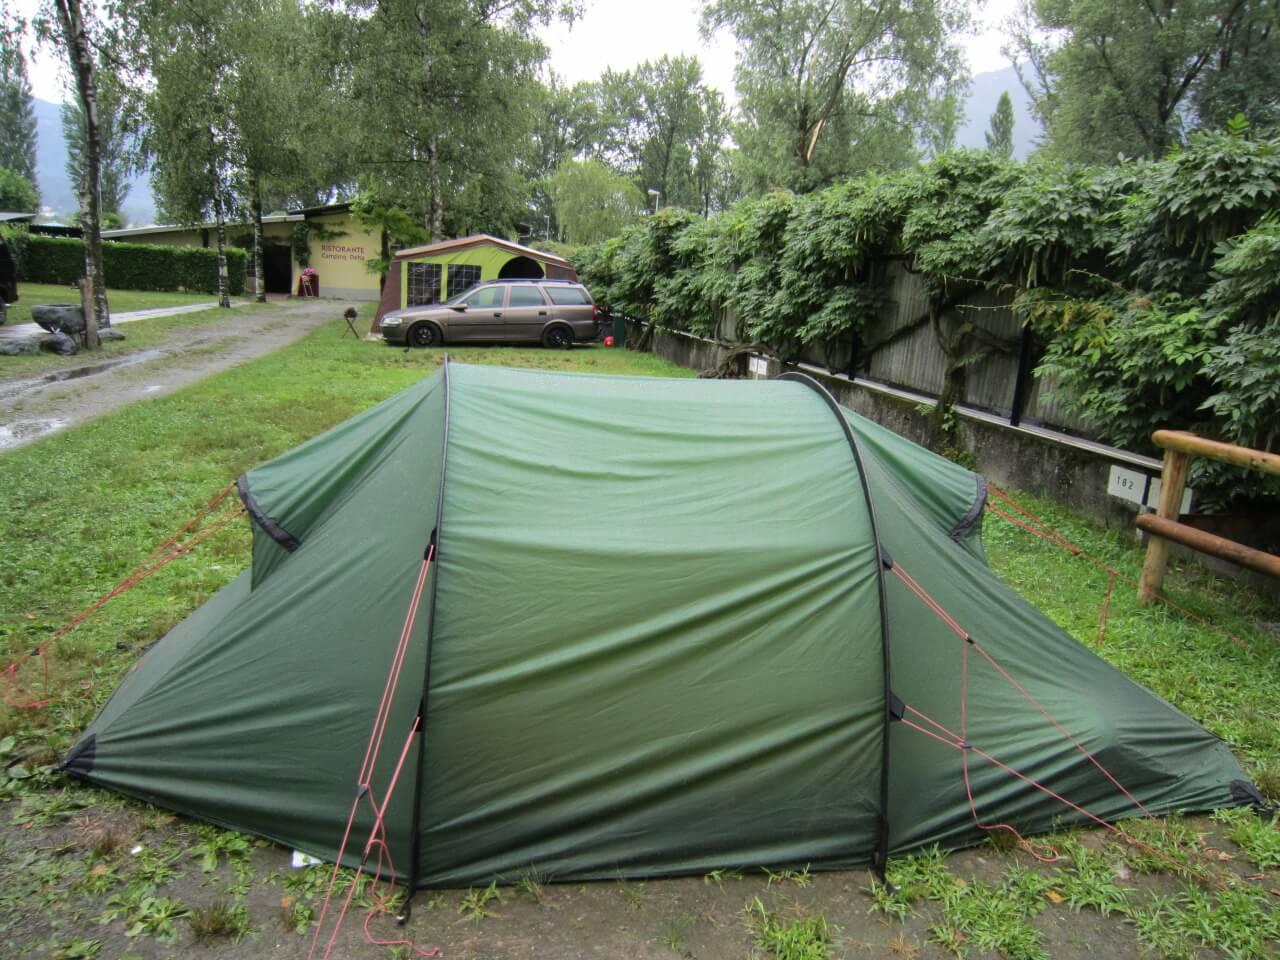
\includegraphics[width=0.6\textwidth]{../Bilder/Locarno/5.jpg}
    \caption{Wasserzelt}
    \label{img:MoonandStars}
\end{figure}

\subsection{Montag 18.07.2011}
Die Sonne blinzelt durch die neuen Vorhänge.
So erwacht man gerne.
Eine kurze doch eher kühle Dusche und schon wurde alles für das Frühstück bereit gemacht.
Nach längerer Suche des Siebes für die Bialleti konnten wir auch einen Kaffee dazu geniessen und die Sonne trocknete das arg gebeutelte Material.
Doch schon wieder waren dunkle Wolken auf dem Weg zu uns.
So beschlossen wir möglichst viel einzupacken und uns dann auf den Weg zurück ins Mittelland zu machen.
Die Rückreise verlief absolut problemlos und die Rückbank war ein weiteres Mal mit schnarchen beschäftigt.
Da wir sowieso über Zürich fuhren konnten wir Michel gerade noch an der Haustüre abliefern und ich konnte noch kurz beim Eglin vorbeischauen um fehlendes Elektromaterial zu besorgen.
Nach der Reinigung des Busses hiess es schon wieder sich auf die Socken nach Stans zu machen, wo am Dienstag der Ernst des Lebens weiterging.
Die kurze Reise ins Tessin und an das Moon \& Stars war ein voller Erfolg und hätte nur durch besseres Wetter übertroffen werden können.
Wer weiss wer nächstes Jahr in Locarno auftreten wird? ...
